\documentclass{article}

\usepackage[parfill]{parskip}
\usepackage[swedish]{babel}
\usepackage{graphicx}

\overfullrule=2cm

\begin{document}

\title{TDDC17: Lab 2}
\author{Henning Hall \& Anton Niklasson}
\maketitle


\section*{Questions}

\section*{In the vacuum cleaner domain in part 1, what were the states and actions? What is the branching factor?}

A state in that world concists of an x position and a y position.

The branching factor for each node ranged between 1 and 4.

\section*{What is the difference between Breadth First Search and Uniform Cost Search in a domain where the cost of each action is 1?}

There is not difference between the two in that situation.

\section*{Suppose that h1 and h2 are admissible heuristics (used in for example A*). Which of the following are also admissible?}
\textbf{a) (h1+h2)/2}

Admissable.

\textbf{b) 2h1}

Not admissable.

\textbf{c) max (h1,h2)}

Admissable.

\section*{If one would use A* to search for a path to one specific square in the vacuum domain, what could the heuristic (h) be? The cost function (g)? Is it an admissible heuristic?}

The heuristic could be the block distance between the current node and the goal node.

The cost function could be something like the total amount of steps from the initial node.

\newpage

\section*{Choose your three favorite search algorithms and apply them to any problem domain.\\Draw the search tree for them, also include the memory usage.}

We constructed a small graph that represents our way home from campus to Ryd. We look at each crossing as a node in the graph.
Below is a sketch of the graph including the cost to move between the nodes:

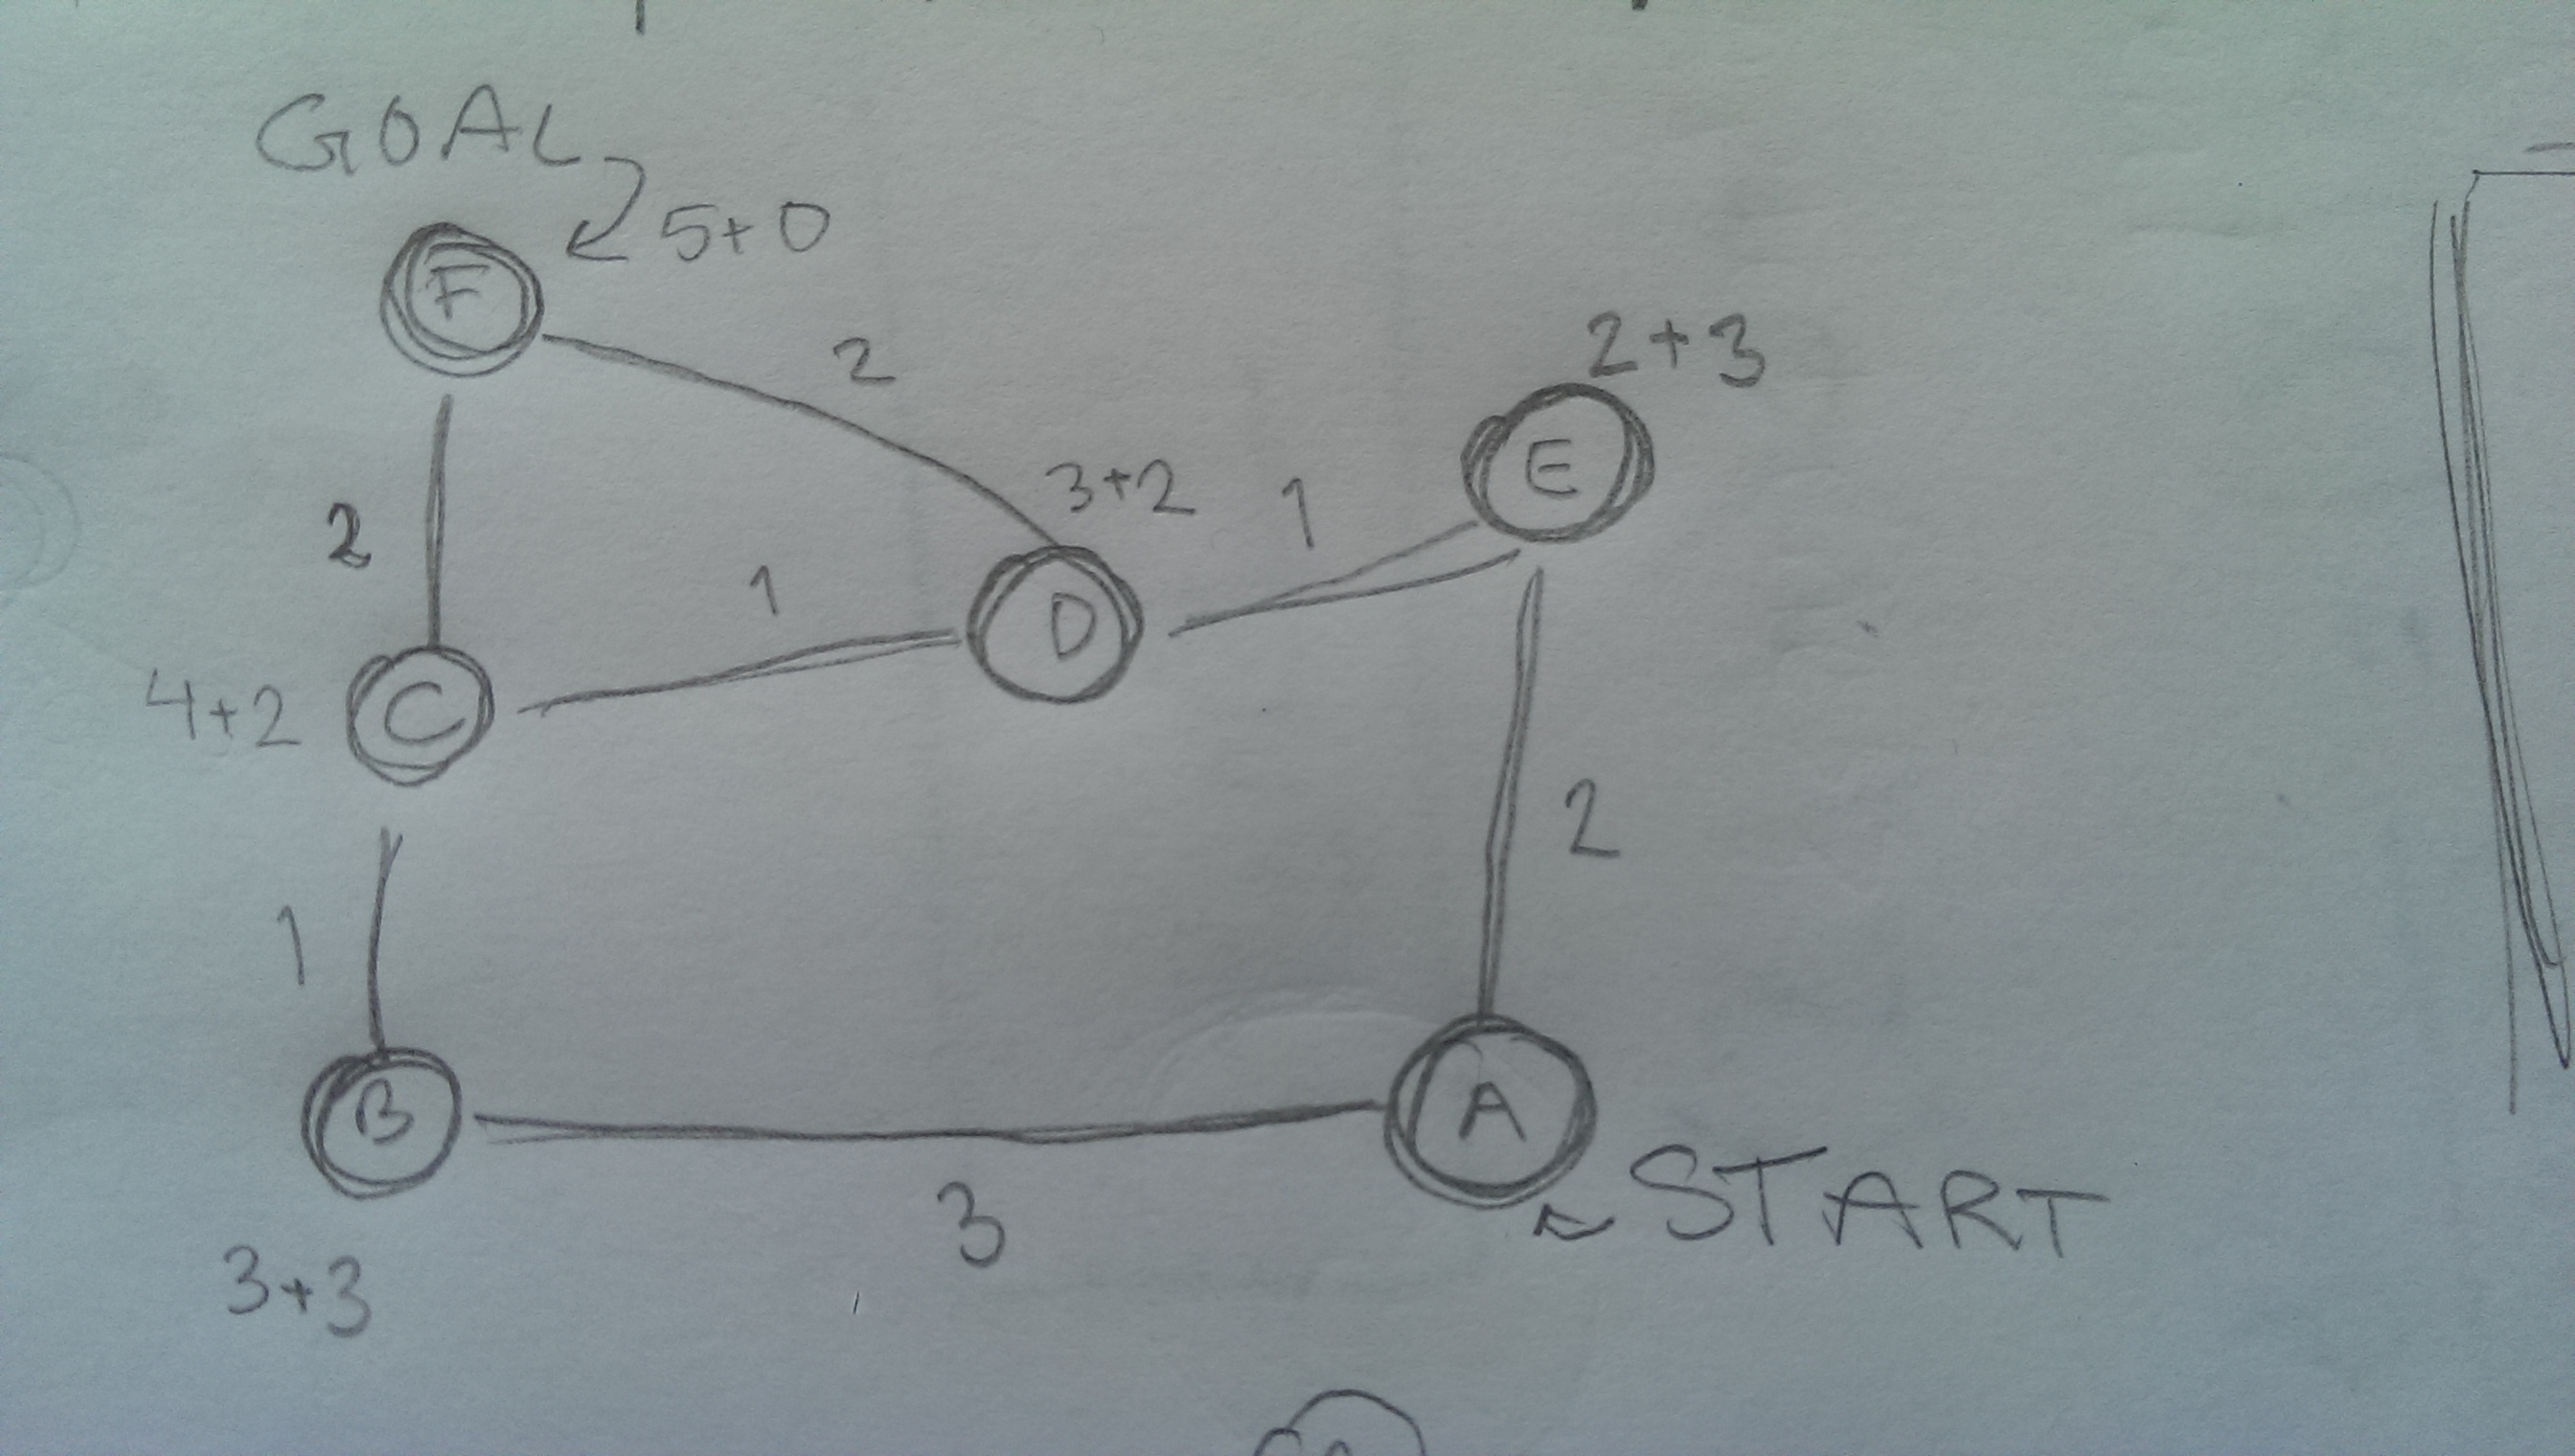
\includegraphics[scale=0.1]{graph}

We start our journey at Karallen which we assigned the letter A. Our apartment is the node F. We chose to look at A*, DFS and BFS.

\subsection*{A* Search}

The table below represents the straight line distance between all the nodes in graph. This table is utilized in our A* heuristic.

\begin{center}
	\begin{table}[h]
		\begin{tabular}{|l|l|l|l|l|l|l|}
			\hline
			   & A 		& B 	& C 	& D 	& E 	& F \\
			\hline
			A  & - 		& 3 	& 3.5	& 3 	& 2 	& 5 \\
			\hline
			B  & 3 		& - 	& 1 	& 1.5 	& 4 	& 3 \\
			\hline
			C  & 3.5	& 1 	& - 	& 1 	& 2 	& 2 \\
			\hline
			D  & 3 		& 1.5 	& 1 	& - 	& 1 	& 2 \\
			\hline
			E  & 2 		& 4 	& 2 	& 1 	& -	 	& 3 \\
			\hline
			F  & 5 		& 3 	& 2 	& 2 	& 3 	& - \\
			\hline
		\end{tabular}
	\end{table}
\end{center}

So, the heursitic \textit{h} is the distance to the goal, and the cost function \textit{g} is the total cost from the start.

Memory usage of the A* algorithm is pretty high. It grows exponentially with the problem which is not ideal.

The main advantage with DFS compared to BFS is that it can be highly space efficient.
By not tracking any visited nodes it is able to use very little memory but that might cause infinite loops.
By tracking visited nodes we prevent infinite loops but we lose that space effiency.

\section*{Look at all the offline search algorithms presented in chapter 3 plus A* search. Are they complete? Are they optimal? Explain why!}

\begin{itemize}
	\item \textbf{Optimal solution} \\
	The solution has the lowest path cost among all solutions.
	\item \textbf{Completness} \\
	Is the algorithm garanteed to find a solution when there is one?
\end{itemize}

\textbf{A* search}\\
It could be both optimal and complete but it depends on h(n). To be optimal if it never oversestimates the cost to reach the goal (admissible heuristic).
If we for example uses the straight line distance as the heuristic it will never overestimate the distance and therefore the algorithm will be optimal. 

\textbf{Breadth-first}\\
It is complete because all nodes will beto the goal node with minimal cost. It might take longer time than A* because it doesn't consider which direction
it is going. As long as the edge cost is positive we believe that it is also complete. 

 visited in the end. It is guranteed optimal only if the step cost is the same since it will return the goal node
with fewest steps from the start.

\textbf{Uniform-cost searc}\\
It is optimal because it finds the path to the goal node with minimal cost. It might take longer time than A* because it doesn't consider which direction
it is going. As long as the edge cost is positive we believe that it is also complete. 

\textbf{Depth-first search}\\
It is not complete because it might be loops in the tree which will make it iterate between nodes. It is not optimal either because it stops at the first
found goal and doesn't investigate other options. 

\textbf{Depth-first search limited}\\
If the search is limited it cant be sure we find the goal, it is therefore not complete and since it is not complete it can't be optimal.

\textbf{Iterative deepening depth-first search}\\
Since it it increasing the depth until the goal is found, the goal will always be found (if we have finite numer of child nodes) and therefore it is complete.
It is optimal if the step cost is the same to each level of nodes. 

\textbf{Bidirectional}
The search will be complete if both sides is using breadth first search and optimal if the step cost is the same. 

\section*{Assume that you had to go back and do lab 1 once more, but this time with obstacles.\\Remember that the agent did not have perfect knowledge of the
environment but had to explore it incrementally.\\Could you still use the search algorithms you have learned to guide the agent's execution?\\What would you search for?}

If we were to solve lab 1 again with obstacles we would try to traverse the world in a depth first manner. We would not really search for anything specific,
the goal would be to keep on traversing until we do not have any unvisited nodes left. We would of course suck up any dust that we find along the way.
When the depth-first traversal is done we transition into an A* search to find our way back home.

\end{document}
